Nadat de kernel in het geheugen geladen is zal deze gestart worden. De Linux kernel zorgt ervoor dat de beschikbare hardware klaar is voor gebruik en dat er processen gestart kunnen worden. Het eerste proces dat de kernel start is \texttt{systemd}\index{systemd}. Vroeger was dit \texttt{init}\index{init} en dat kan je op vele ander Unix-achtige besturingssystemen nog tegen komen, maar de meeste Linux distributies zijn over naar \texttt{systemd}.

\texttt{systemd} is het proces dat ervoor zorgt dat alle ander processen gestart worden. De \texttt{systemd} daemon heeft proces nummer 1. Het is de eerste daemon die start bij het opstarten van het systeem en de laatste die afgesloten wordt bij het afsluiten van het systeem.

Naast de \texttt{systemd} daemon die de moeder is van alle processen, zijn er ook commando's waarmee je (als root) daemons kunt starten, stoppen en herstarten. Het commando dat doorvoor beschikbaar is heet \texttt{systemctl}\index{systemctl}. Een standaard met de installatie meegekomen daemon in de systemd-timesyncd\index{timesyncd}\index{systemd!timesyncd} daemon. We gaan deze daemon gebruiken om een beetje vertrouwd te raken met \texttt{systemctl}.

\begin{lstlisting}[language=bash]
sudo systemctl status systemd-timesyncd
\end{lstlisting}

\begin{figure}[h]
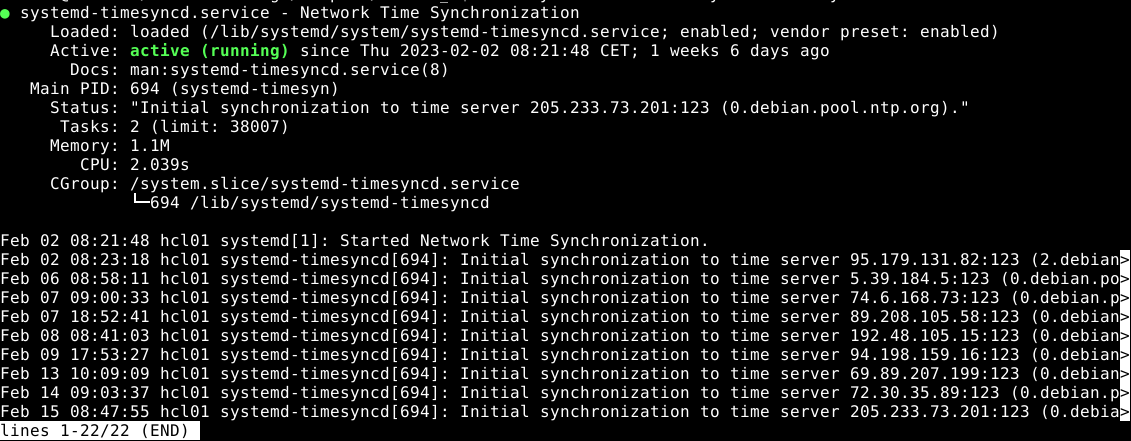
\includegraphics[width=8cm]{systemd-timesyncd-status}
\centering
	\caption{Status output van systemctl}
	\label{scrn:systemd-timesyncd-status}
\end{figure}

Als je net als in het voorbeeld (Figuur \ref{scrn:systemd-timesyncd-status}) een lijn hebt met END dan kan je gebruik maken van 'q' om weer op de command-prompt terecht te komen.

Door aan \texttt{systemctl} de commando's stop of start mee te geven kunnen we daemons op ons systeem stoppen en starten. De tijd synchronisatie daemon is op dit moment gestart, dus het eerste wat we kunnen doen is hem stoppen:

\begin{lstlisting}[language=bash]
sudo systemctl stop systemd-timesyncd
\end{lstlisting}

Met \texttt{systemctl status} kunnen nu de status van de daemon zien en dan zien we dat deze gestopt is. Het opnieuw opstarten doen we met start:

\begin{lstlisting}[language=bash]
sudo systemctl start systemd-timesyncd
\end{lstlisting}

